\documentclass{article}
\usepackage{graphicx}
\usepackage{fullpage}
\usepackage{dirtree}
\usepackage[most]{tcolorbox}
\usepackage{parskip}
\usepackage{wrapfig}      
\usepackage{tcolorbox}
\usepackage{enumitem}
\usepackage{listings}
\usepackage{color}
\usepackage{subcaption}
\usepackage{hyperref}



\usepackage{tikz}
\usepackage{etoolbox} % for \ifnumcomp
\usepackage{listofitems} % for \readlist to create arrays

\tikzset{>=latex} % for LaTeX arrow head
\colorlet{myred}{red!80!black}
\colorlet{myblue}{blue!80!black}
\colorlet{mygreen}{green!60!black}
\colorlet{mydarkred}{myred!40!black}
\colorlet{mydarkblue}{myblue!40!black}
\colorlet{mydarkgreen}{mygreen!40!black}
\tikzstyle{node}=[very thick,circle,draw=myblue,minimum size=22,inner sep=0.5,outer sep=0.6]
\tikzstyle{connect}=[->,thick,mydarkblue,shorten >=1]
\tikzset{ % node styles, numbered for easy mapping with \nstyle
  node 1/.style={node,mydarkgreen,draw=mygreen,fill=mygreen!25},
  node 2/.style={node,mydarkblue,draw=myblue,fill=myblue!20},
  node 3/.style={node,mydarkred,draw=myred,fill=myred!20},
}
\def\nstyle{int(\lay<\Nnodlen?min(2,\lay):3)} % map layer number onto 1, 2, or 3


\definecolor{dkgreen}{rgb}{0,0.6,0}
\definecolor{gray}{rgb}{0.5,0.5,0.5}
\definecolor{mauve}{rgb}{0.58,0,0.82}

\lstset{frame=tb,
  language=C,
  aboveskip=3mm,
  belowskip=3mm,
  showstringspaces=false,
  columns=flexible,
  basicstyle={\small\ttfamily},
  numbers=none,
  numberstyle=\tiny\color{gray},
  keywordstyle=\color{blue},
  commentstyle=\color{dkgreen},
  stringstyle=\color{mauve},
  breaklines=true,
  breakatwhitespace=true,
  tabsize=3
}




% \tikzset{%
%   every neuron/.style={
%     circle,
%     draw,
%     minimum size=1cm
%   },
%   neuron missing/.style={
%     draw=none, 
%     scale=4,
%     text height=0.333cm,
%     execute at begin node=\color{black}$\vdots$
%   },
% }


\begin{document}

\title{C Project Final Report}
\author{Baray Efe Rafioglu, Azra Nesrin Ayer, Rohan Choudhary, Ege Hurturk}
\date{June 20, 2025}


\maketitle

\section{Assembler}
\subsection{Assembler Structure}

\begin{itemize}
    \item \verb|assemble_utils.c/.h|: It contains helper functions to be used around the file. \verb|create_empty_file|, \verb|load_file| and \verb|print_instructions_to_binary| help with file I/O, \verb|resolve_alias_mnemonic| normalizes alias mnemonics; and \verb|string_to_immediate| converts numeric strings to integers. And the header file declares the functions to be used through the folder.

\item \verb|assemble.c|: It is the entry point for the assembler. It first parses command-line arguments to get the input and output files, then implements a two-pass assembly process. In the first pass, it initializes a symbol table and calls \verb|fill_symbol_table|: which populates the table with labels and their corresponding memory addresses. In the second pass, it calls the parser to tokenise the source file, build an array of instruction representations, and calls the relevant instruction encoding functions to encode instructions. Finally, it writes the binary output to the specified file or standard output.
\item \verb|encoding_functions.c|: It contains all the binary decoding functions for different types of instructions: \verb|encode_dp_immediate|, \verb|encode_dp_register|, \verb|encode_multiply|, \verb|encode_wide_move|, \verb|encode_branch|,\\ \verb|encode_load_store| and \verb|encode_directive|. The function \verb|encode_instructions| selects the right encoding function by \verb|instruction_t|. It also contains static lookup tables different mnemonics. The header file additionally has helper structs such as \verb|general_entry| to be used in the source file.

\item \verb|instruction_representation.c|: It contains functions that constructs and frees the struct \verb|instruction_t|. 

\item \verb|instruction_representation.h|: It defines enums for instruction types, addressing modes, and condition codes. \verb|instruction_t| is the main struct that represents an assembly instruction, holding its mnemonic, type, registers, operands and instruction specific fields. 

 \item \verb|parser.c/.h|: It is the file that handles the parsing of source file. It defines the \verb|parser_state_t| struct to manage parsing process and store essential info regarding the assembly program. It then converts the source file to tokens, and eventually parses it to \verb|instruction_t| and sets instruction type based on instruction mnemonic.

\item \verb|symbol_table.c/.h|: It is a dynamic symbol table that stores labels and their addresses. \\ \verb|symbol_table_create()| initializes a new, empty symbol table. \verb|symbol_table_append()| adds a new label address pair to the table. \verb|symbol_table_find()| checks if a label exists in the table. \verb|symbol_table_get()| searches for a label in the table and returns its address. These functions were useful to store labels in first pass.
    
\item \verb|storing_labels.c|: It handles the first pass of the program. It goes through the input file and maps label names to their corresponding addresses via a \verb|symbol_table|.

\item \verb|tokens.c/.h| It contains useful functions to tokenise the input file. The \verb|token_t| struct and the \verb|token_type_t| enum  represents all possible tokens (registers, immediates, mnemonics, labels, literal, shift, "[" , "]", "!",  directives, new lines and end of the files. The \verb|tokenise()| function reads the source code and breaks it into a list of these tokens. The tokenisation process is useful because it makes parsing easier and makes the language extendible.
\end{itemize}



\subsection{Assembler Implementation}

We performed two passes over the source code to implement our assembly.
\begin{itemize}
    \item During the first pass, our assembler scans through the assembly code to collect all labels and their corresponding memory addresses. To store this information, we created \verb|symbol_table| using hashmap structure where each label, a string, is mapped to its associated memory address, an unsigned integer. In order to keep the access and updating of the hashmaps as efficient as possible we hashed the strings and used buckets which doubled in amount every time the element amount in the hashmap exceeded 0.75 times the amount of buckets. For the string hashing, we used a polynomial rolling hash function and set the base ($p$) to be 255 and the modulus to be the natural \textbf{uint\_64} limit.
$$
hash(s) = s[0] + p s[1] + p^2 s[2] + \dots + p^{(n-1)} s[n - 1]
        = \sum^{n - 1}_{i=0} p^i s[i]
$$
We have also implemented and tested a freeing method that safely frees all memory occupied by the hashmap.

    \item In the second pass, our assembler translates the assembly code into 32 bit machine code, using the \verb|symbol_table| it created in the first pass. This process involves tokenizing the source code, parsing the instructions into the type \verb|instruction_t| and later encoding them into binary representation. Our assembler handles label references using our \verb|symbol_table|. During encoding, errors such as undefined labels, invalid mnemonics and immediate values that are out of range are reported and then handled by setting the binary encoding to 0. Once all instructions are encoded, we write them to the output file in little endian format.
\end{itemize}
\\

\begin{figure}[h!]
    \centering
    \includegraphics[width=\linewidth]{flow.png}
    \caption{Workflow for assembler}
    \label{fig:mnist-digits}
\end{figure}




\section{Part 3: Raspberry Pi Implementation}

After making sure that our assembler and emulator works correctly using the tests, we wrote an assembly code where we implemented the following steps:
\begin{itemize}
    \item We first initialized the 7th pin as the output pin, which was done by loading the base address of the GPIO Function Select registers into a register and then by calculating the appropriate offset setting the 7th pin as the output pin.
    \item After that, we turned on the LED by loading the base address of GPIO Output Set registers to a register and similarly, calculating to appropriate offset to set the 7th pin high.
    \item Later, we implemented a delay to create a visible blinking effect. This was done by decrementing a counter until it reaches 0.
    \item We then turned off the LED by setting the 7th to a low signal in a similar way that was described before by setting the pin to GPIO Output Clear.
    \item After turning the LED off, we then make another delay and jump back to the place where we turn on the LED and hence create a constant blinking effect.
\end{itemize}


\section{Part 4: Extention}
\subsection{Detailed Description}
As a part of the project, we implemented a neural network from scratch in C to recognize handwritten MNIST digits, and integrated it with a graphics interface and Raspberry Pi hardware.
\subsubsection{Neural Network}
To represent a neural network in C, we designed two core data structures: one for individual layers, and one for the full model:
\begin{lstlisting}
// Represents a fully connected layer in the neural network.
typedef struct {
    int size;                       // Number of neurons in this layer
    double *activations;            // Output activations for this layer, f(z)
    double *z_values;               // Pre-activation values (Wx + b)
    double *biases;                 // Biases for each nuron in this layer
    
    double **weights;               // Weight matrix: [size][prev_size]
    double *deltas;                 // Backpropagation deltas
    double **grad_weights;          // Gradient of weights
    double *grad_biases;            // Gradient of biases
} layer;

// Represents the entire neural network model.
typedef struct {
    int num_hidden_layers;
    layer *hidden_layers;

    layer output_layer;

    double *input; // INPUT_SIZE
} model_t;
\end{lstlisting}
Each layer stores the neuron activations, biases, and weight matrix connecting it to the previous layer. It also stores intermediate values needed for backpropagation (such as deltas and gradients). This structure allows us to flexibly model a fully connected multi-layer perceptron with any number of hidden layers.
We implemented key functions to perform training:

\begin{enumerate}
    \item \texttt{model\_forward}: Performs a forward pass, computing activations for all layers based on input.
    \item \texttt{model\_backward}: Computes gradients of loss with respect to weights and biases using backpropagation.
    \item \texttt{model\_update}: Updates weights and biases using the computed gradients and a specified learning rate.
    \item \texttt{model\_predict} Performs inference and computes the output predictions for a given input.
\end{enumerate}
\begin{figure}[h!]
\centering

% NEURAL NETWORK
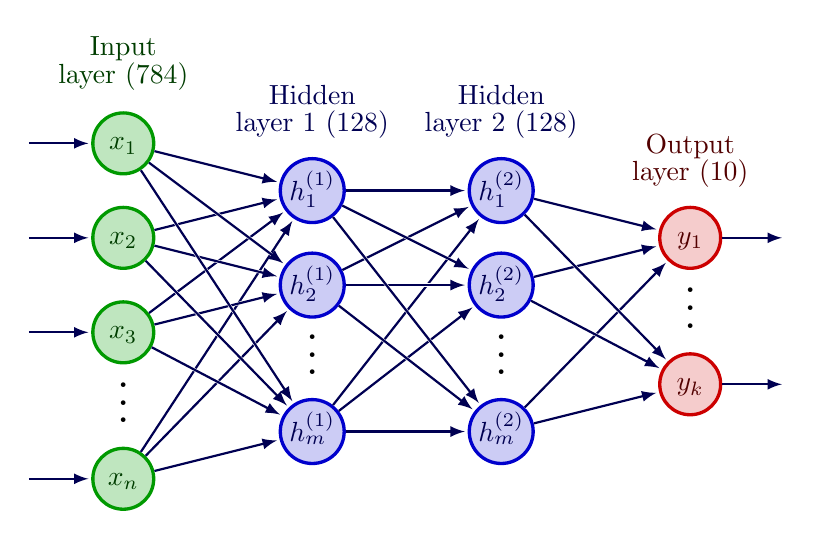
\begin{tikzpicture}[x=2.4cm,y=1.2cm]
  \readlist\Nnod{4,3,3,2} % array of number of nodes per layer
  \readlist\Nstr{n,m,k} % array of string number of nodes per layer
  \readlist\Cstr{x,h^{(\prev)},y} % array of coefficient symbol per layer
  \def\yshift{0.55} % shift last node for dots
  
  % LOOP over LAYERS
  \foreachitem \N \in \Nnod{
    \def\lay{\Ncnt} % alias of index of current layer
    \pgfmathsetmacro\prev{int(\Ncnt-1)} % number of previous layer
    \foreach \i [evaluate={\c=int(\i==\N); \y=\N/2-\i-\c*\yshift;
                 \x=\lay; \n=\nstyle;
                 \index=(\i<\N?int(\i):"\Nstr[\n]");}] in {1,...,\N}{ % loop over nodes
      % NODES
      \node[node \n] (N\lay-\i) at (\x,\y) {$\strut\Cstr[\n]_{\index}$};
      
      % CONNECTIONS
      \ifnumcomp{\lay}{>}{1}{ % connect to previous layer
        \foreach \j in {1,...,\Nnod[\prev]}{ % loop over nodes in previous layer
          \draw[white,line width=1.2,shorten >=1] (N\prev-\j) -- (N\lay-\i);
          \draw[connect] (N\prev-\j) -- (N\lay-\i);
        }
        \ifnum \lay=\Nnodlen
          \draw[connect] (N\lay-\i) --++ (0.5,0); % arrows out
        \fi
      }{
        \draw[connect] (0.5,\y) -- (N\lay-\i); % arrows in
      }
      
    }
    \path (N\lay-\N) --++ (0,1+\yshift) node[midway,scale=1.6] {$\vdots$}; % dots
  }
  
  % LABELS
  \node[above=4,align=center,mydarkgreen] at (N1-1.90) {Input\\[-0.2em]layer (784)};
  \node[above=3,align=center,mydarkblue] at (N2-1.90) {Hidden\\[-0.2em]layer 1 (128)};
  \node[above=3,align=center,mydarkblue] at (N3-1.90) {Hidden\\[-0.2em]layer 2 (128)};
  \node[above=3,align=center,mydarkred] at (N\Nnodlen-1.90) {Output\\[-0.2em]layer (10)};
  
\end{tikzpicture}
\caption{Architecture of the 2-layer neural network trained to recognize MNIST images.}
\label{fig:neural-network}
\end{figure}

Our neural network architecture has 4 layers, consisting of an input layer of 784 nodes ($28 \cdot 28$ images), 2 hidden layers with 128 nodes, and an output layer of 10 nodes.

For the hidden layers, we used the sigmoid activation function:
$$
\sigma(x) = \frac{1}{1+e^{-x}}
$$
At the output layer, to perform multi-class classification (digits 0–9), we used the softmax activation function:
$$
\text{softmax}(z_i)=\frac{e^{z_i}}{\sum_j e^{z_j}}
$$
\subsubsection{Data}
We wrote a dedicated data loading module in \texttt{data\_loader.c/h}, designed to parse the MNIST dataset files and structure the data for training:

\begin{lstlisting}
// Represents a collection of images and their corresponding labels
// Each image is stored as an array of 784 doubles (normalized grayscale [0,1]), and labels are stored as `uint8_t` digits (0 to 9).
typedef struct {
    double **images;    // Normalized [0,1]
    uint8_t *labels;    // Raw digit labels (0-9)
    int size;
} dataset;
\end{lstlisting}
We implemented several functions in this module, including \texttt{read\_mnist\_images}, which reads raw image data from MNIST \texttt{.idx3-ubyte} files into memory, \texttt{load\_dataset}, which loads both images and labels into a \texttt{dataset} struct, \texttt{split\_dataset}, which splits a dataset into training and testing subsets based on a provided ratio. Other functions can be found in our GitLab \footnote{\url{https://gitlab.doc.ic.ac.uk/lab2425_summer/armv8_27}} repository.
\end{enumerate}

\subsection{User Interface}
On the user interface part of the extension we used the SDL2 library on C. We created a 28x28 grid with \textbf{uint8\_t} values in each cell and assigned 255 to each cell at the start of the program to make the whole grid white. When the mouse is pressed the cell it is on turns black. We can also reset the whole grid to white by pressing x.
One issue we have faced during the creation of the UI was that the mouse trail would skip a lot of cells in between frames leading to separate dots on the grid if the user moved the mouse too fast. To fix this issue we took the previous location of the mouse and filled in the cells in between the old location and the new one every frame.

\subsection{Raspberry Pi}
To display our code on the Raspberry Pi, we first downloaded Operating Systems to our Raspberry Pi, later we connected it to our monitor and wrote a python code to run on it. The code takes the predicted digit as an input and in every 0.5 seconds converts the digit from decimal to binary. We also connected 4 LED lights to a breadboard and connected it to our Raspberry Pi so that binary representation can be represented with the lighting of the corresponding LEDs.

\subsection{Challenges}
During the extension, our team faced with lots of challenges. These challenges primarily stem from training the neural network, where the MNIST images in the training dataset do not match the images that we capture from the grid in the app. To make them resemble each other, we applied a $3\cdot3$ box blur and we centered the digits drawn on the grid. Plus, the digits in the MNIST dataset were big, so we made the brush 3x3 instead of 1x1. Figure \ref{fig:combined} displays the image captured from the grid after preprocessing and a sample image of the digit 8 from the MNIST dataset.

\begin{figure}[h!]
    \centering
    \makebox[0.7\linewidth]{ % adjust this value to control horizontal positioning
        \begin{subfigure}{0.25\linewidth}
            \centering
            \includegraphics[width=\linewidth]{digit3.png}
            \caption{Image drawn}
            \label{fig:sub1}
        \end{subfigure}
        \hfill
        \begin{subfigure}{0.3\linewidth}
            \centering
            \includegraphics[width=\linewidth]{dig8.png}
            \caption{Sample MNIST image}
            \label{fig:sub2}
        \end{subfigure}
    }
    \caption{Comparison of the two images.}
    \label{fig:combined}
\end{figure}

\subsection{Testing Extention}
We have tested our implementation manually, where we tried to give our program a lot of numbers to predict and see if it does give the result that it should be giving. We looked for patterns in any mistakes it made and used that to understand how accurate and reliable it was. The testing method was helpful for debugging and small scale execution however we think it is not the most efficient way to test the entire program as it can't handle every possible case. The testing we did was helpful for us but there is room to thoroughly check our code with bigger testing data in the future.


\section{Group Reflecion}
We had great communication, as we always did peer programming during lab sessions and used VSCode Live Share. Everyone was active in the sessions and participated in group communication through WhatsApp. During our time working on this project, we shared the responsibility of tasks equally among ourselves, ensuring that each team member contributed. Our reasoning was that dividing tasks evenly would maximize efficiency, helping us meet the deadline with ease while also producing the best possible code. Although we worked on separate parts of the project, we made sure to share our progress and exchange ideas with each other. Next time, we might aim to start a bit earlier, as we ran short on time toward the end. However, we’ll definitely maintain the same level of communication, as it helped us make steady progress throughout the project.



\section{Individual Reflection}
\subsection{Baray Efe Rafioglu}
Working on this project taught me invaluable collaboration skills in software engineering. I had never used Git before, and learning it with my teammates significantly improved my ability to manage code and work in a team without conflicts. A key piece of feedback I received was about misreading specifications, which sometimes led to bugs—like reversing return values in a flag function. I’ve since made it a priority to fully understand the spec before writing code. On the upside, when I grasped the task well, I was quick to find effective solutions. This led me to focus on more abstract and algorithm-heavy parts of the project, like building the hashmap for the assembler and writing the emulator’s flag functions. Overall, this project helped me grow both technically and as a team player, while giving me firsthand experience in coding practices and professional workflows.


\subsection{Azra Nesrin Ayer} 
Through this project, I gained a better understanding of what it means to be part of a team. In the past, I was more used to working independently and handling every aspect of it on my own so adapting to work as a team member was a valuable experience for me. I did find it challenging at times to ask for help because I was not used to doing it. I will try to be more open to reaching out when I need support in my future projects. Additionally, I believe I was a reliable team member who did tasks on time which are some things that I want to maintain on my next projects. I also learned a lot about C and got to practise using Git in a professional setting.

\subsection{Rohan Choudhary}
The project was a great opportunity to strengthen my group work skills. Having worked in teams before, I felt confident in my communication abilities, but this project offered a new kind of experience and taught me a lot about collaborating on software development within a team environment. My previous experience helped the group work effectively. I made a conscious effort to regularly discuss ideas and ensure everyone remained aligned throughout the development process. On the technical side, the project was challenging. I had to learn and adapt to new tools and workflows, especially Git, which I hadn’t used before. It also helped me develop a solid understanding of C, and adopt good software development paradigms. Our extension provided an even tougher challenge, by invloving both software and hardware. It deepened my understanding of the Raspberry Pi and gave me hands-on experience with integrating physical components with our code. Overall, it was a rewarding experience that taught me a great deal about writing reliable software as part of a team.

\subsection{Ege Hurturk}
Throughout this project, I contributed to multiple parts of the system, which gave me a chance to develop new skills across both low-level and high-level programming. Working on the emulator strengthened my understanding of ARMv8 architecture and bit-level encoding of instructions. In the assembler, I implemented the parsing logic and the instruction encoding pipeline — this was particularly challenging, and it helped me to understand how a compiler works. It was particularly challenging as it required careful handling of binary formats and precise control over token operations such as \texttt{advance(token\_list\_t)} 'ing the token list.  For the extension, I got to put my skills in AI into practice, writing a neural network library from scratch in C. Finally, connecting the network to Raspberry Pi GPIOs and controlling LEDs to display predictions was an exciting challenge in hardware-software integration. Overall, this project broadened my skills in C programming, embedded systems, and machine learning, and taught me valuable lessons in working in a team and using Git effectively.



\end{document}
